% !TEX root = praca.tex

\chapter{Implementacja rozpraszania zadań}
\label{chap:impl}
Poniższy rozdział został poświęcony szczególnie istotnym aspektom implementacyjnym biblioteki umożliwiającej uruchamianie zadań na wielu różnych komputerach w języku Haskell, ze szczególnym uwzględnieniem dodatkowych bibliotek i rozszerzeń tego języka.

\section{Broker RabbitMQ}
\textbf{RabbitMQ} to otwartoźródłowy broker wiadomości - oprogramowanie zapewniające odporny na zakłócenia mechanizm komunikacji sieciowej. Został zaimplementowany w języku Erlang z wykorzystaniem Open Telecom Platform. Posiada biblioteki dla wszystkich znaczących języków programowania - w tym dla Haskella (biblioteka amqp - od ang. Advanced Message Queuing Protocol). Dwie najważniejsze koncepcje implementowane przez RabbitMQ to - \textbf{kolejki} (ang. queues) oraz \textbf{wymienniki} (ang. exchanges). Kolejki to przetrzymywane przez serwer struktury FIFO z sieciowym protokołem dostępu. Są najbardziej podstawową abstrakcją stosowaną w rozproszonym programowaniu współbieżnym, a w przypadku projektu będącego przedmiotem tej pracy pozwalają wielu węzłom ''konkurować'' o zadania w bezpieczny sposób (nigdy nie dojdzie do sytuacji, w której dwa zadania są w tym samym czasie wykonywane na dwóch różnych węzłach). Wymienniki są pośrednikami dostępu do zbiorów kolejek - wiadomość, która zostanie dodana do wymiennika może zostać powielona i rozdystrybuowana do połączonych z wymiennikiem kolejek w jeden z czterech możliwych sposobów zależnie od predefiniowanego typu wymiennika:
\begin{description}[align=right,labelwidth=3cm,leftmargin=3cm]
  \item [direct] wiadomość trafia tylko do kolejek z określonym kluczem routującym, identycznym z kluczem zawartym w nagłówku wiadomości
  \item [fanout] wiadomość trafia do wszystkich podłączonych kolejek
  \item [topic] wiadomość trafia do konkretnej kolejki tylko wtedy, kiedy jej klucz routujący spełnia wzorzec określony dla tej kolejki 
  \item [headers] wiadomość trafia do konkretnej kolejki na podstawie innych niż klucz routujący parametrów zawartych w nagłówku
\end{description}

Topologia wykorzystywana w projekcie zakłada, że każdy węzeł może nasłuchiwać więcej niż jednej kolejki zadaniowej (jest to pożądane w przypadku kiedy nie każdy węzeł jest w~stanie obsłużyć każdy typ zadania). Dodatkowo każdy węzeł tworzy własną kolejkę na zlecenia przerwania zadania i przypina ją do wspólnego wymiennika typu \lstinline{fanout}. Gwarantuje to dostarczenie każdemu węzłowi komunikatu przerwania niezależnie od awarii komunikacji z brokerem. Topologia kolejkowania została przedstawiona na rysunku \ref{fig:topo}.

\begin{figure}[h]
\resizebox{\textwidth}{!}{%
\input{komunikacja.tikz}
}%
\caption{Topologia kolejkowania}
\label{fig:topo}
\end{figure}

\section{Zarządzanie zasobami}
Protokół AMQP operuje na zależnych od siebie zasobach, którymi należy w poprawny sposób zarządzać. Postawowy przykład z dokumentacji biblioteki AMQP (Listing \ref{lst:conn}), w przypadku wystąpienia wyjątku nie gwarantuje zwolnienia zasobu, a kolejność wykonywania finalizatorów ze względu na leniwą ewaluację jest determinowana wyłącznie wyzwoleniem mechanizmu odśmiecania.

\begin{lstlisting}[caption=Łączenie z RabbitMQ, label=lst:conn]
main = do
  conn <- openConnection "127.0.0.1" "/" "guest" "guest"
  ...
  closeConnection conn
\end{lstlisting}

Jednym z istniejących rozwiązań tego problemu jest biblioteka \texttt{io-region} \cite{IoReg}, umożliwiająca podział kodu na regiony odpowiedzialne za poszczególne zasoby (Listing \ref{lst:reg}) oraz przenoszenie tych odpowiedzialności pomiędzy regionami.
\begin{lstlisting}[caption=Regionalizacja zasobów, label=lst:reg]
...
region $ \r -> do
 connection <- alloc_ r (AMQP.openConnection host vhost username password)
                         AMQP.closeConnection
  -- po opuszczeniu regionu następuje zwolnienie zasobów
...
\end{lstlisting}

Rejestrowanie zasobów w obrębie odpowiednich regionów rozwiązuje również problem asynchronicznych wywołań zwrotnych, służących do obsługi nadchodzących komunikatów z brokera. Dla porównania, niewłaściwe rozwiązanie oparte o mechanizm \lstinline{bracket} (przedstawione na listingu \ref{lst:brac}) powoduje przedwczesne zamknięcie zasobu nadal wykorzystywanego przez funkcję uruchamianą asynchronicznie.
\begin{lstlisting}[caption=Problem funkcji asynchronicznych, label=lst:brac]
...
bracket openConnection closeConnection $ \connection ->
  bracket (openChannel connection) closeChannel $ \channel1 ->
    consumeMsgs channel1 queue callback -- wywołanie asynchroniczne
  -- nieporządane zamknięcie kanału
  -- otwarcie drugiego kanału
  bracket (openChannel connection) closeChannel $ \channel2 ->
    consumeMsgs channel2 queue callback -- wywołanie asynchroniczne
    -- nieporządane zamknięcie kanału
  _ <- getLine -- oczekiwanie
-- zamknięcie połączenia

...
region $ \r -> do
  connection <- alloc_ r openConnection closeConnection
  channel1 <- alloc_ r (openChannel connection) closeChannel
  consumeMsgs channel1 queue callback
  channel2 <- alloc_ r (openChannel connection) closeChannel
  onsumeMsgs channel2 queue callback

  _ <- getLine -- oczekiwanie
  -- zwolnienie zasobów w poprawnej kolejności
\end{lstlisting}
\newpage

\section{Środowisko funkcji}
Większość funkcji związanych z protokołem AMQP wymaga do działania przekazania pewnego zasobu (jak na przykład obiekt \lstinline{Connection} lub \lstinline{Channel}). Robienie tego za każdym razem explicite prowadzi do zmniejszenia czytelności kodu. Idiomatycznym dla języka Haskell rozwiązaniem jest zastosowanie przedstawionego na listingu \ref{lst:reader} typu \lstinline{Reader} \cite{Reader}.
\begin{lstlisting}[caption=Typ reader, label=lst:reader]
newtype Reader e a = Reader { runReader :: e -> a }

instance Functor (Reader e) where
  fmap f r = Reader $ \e -> f (runReader r e)

instance Applicative (Reader e) where
  pure a    = Reader $ \e -> a
  ra <*> rb = Reader $ \e -> (runReader ra e) (runReader rb e)

instance Monad (Reader e) where 
  (Reader r) >>= f = Reader $ \e -> runReader (f (r e)) e

ask :: Reader a a
ask = Reader id
\end{lstlisting}

Typ \lstinline{Reader} opakowuje funkcję przyjmującą jako argument środowisko jej wykonania i zwracającej pewien wynik obliczeń wykorzystujących to środowisko. Przykładowo dla:

\begin{lstlisting}
testReader :: Reader Bool String
testReader = Reader $ \flag -> if flag then "Włącz" else "Wyłącz"
\end{lstlisting}
wywołanie \lstinline{runReader testReader True} zwróci wartość \lstinline{"Włącz"} -- jednak istotą działania \lstinline{Reader}'a jest jego monadyczny interfejs umożliwiający zapisanie funkcji \lstinline{testReader} jako:

\begin{lstlisting}
testReader :: Reader Bool String
testReader = do
  flag <- ask
  return $ if flag then "Włącz" else "Wyłącz"
\end{lstlisting}

Dzięki temu unikamy przekazywania tego samego środowiska za każdym razem jako argumentu funkcji, co jest szczególnie istotne w przypadku kiedy jest to wiele funkcji.

Niestety funkcjonalność samej monady \lstinline{Reader} nie jest wystarczająca ze względu na mnogość operacji wykorzystujących operacje wejścia-wyjścia, więc wymagających typu \texttt{IO} do działania. Pomocne okazują się przedstawione na listingu \ref{lst:transformers} transformatory monad (ang.~\textit{Monad transformers} \cite{Transformers}):

\begin{lstlisting}[caption=Transformator typu Reader, label=lst:transformers]
newtype ReaderT e m a = ReaderT { runReaderT :: e -> m a }

instance Functor m => Functor (ReaderT e m) where
  fmap f r = ReaderT $ \e -> fmap f (runReaderT r e)

instance Applicative m => Applicative (ReaderT e m) where
  pure a    = ReaderT $ \e -> pure a
  ra <*> rb = ReaderT $ \e -> (runReaderT ra e) <*> (runReaderT rb e)

instance Monad m => Monad (ReaderT e m) where 
  r >>= f = ReaderT $ \e -> do
    a <- runReaderT r e
    runReaderT (f a) e

ask :: Monad m => ReaderT a m a
ask = ReaderT return

lift :: m a -> ReaderT e m a
lift m = ReaderT (const m)
\end{lstlisting}
Dzięki funkcji \lstinline{lift} możemy niejako ,,podciągać'' operacje wykonane w ramach innej monady do typu \lstinline{ReaderT}:

\begin{lstlisting}
testReader :: ReaderT Bool IO String
testReader = do
  flag <- ask 
  lift $ if flag then putStrLn "Włącz"
                 else putStrLn "Wyłącz"
  return "Wynik"

> runReaderT testReader True
Włącz
\end{lstlisting}

\newpage
\section{Odczyt konfiguracji z pliku}
Biblioteka \texttt{configurator} \cite{Conf} umożliwia odczyt plików konfiguracyjnych i zapewnia uproszczony interfejs dostępu do przechowywanych wewnątrz wartości parametrów, a w przypadku ich braku korzysta z wartości domyślnej zapisanej ,,na sztywno'' w kodze konfigurowanego programu, co dla poniższego (\ref{lst:config}) pliku konfiguracyjnego zostało zaimplementowane na listingu~\ref{lst:configuse}.
\begin{lstlisting}[caption=Przykładowy plik konfiguracyjny, label=lst:config]
taskell {
  rabbitmq {
    host     = "localhost"
    vhost    = "/"
    username = "guest"
    password = "guest"
  }
  abortExchange = "taskell.abort"
  parallelism = 1
  queues = ["taskell.q1", "taskell.q2"]
}
\end{lstlisting}

\begin{description}[align=right,labelwidth=10cm,leftmargin=6cm]
  \item[taskell.rabbitmq.host] Nazwa sieciowa lub adres IP brokera
  \item[taskell.rabbitmq.vhost] URL hosta wirtualnego
  \item[taskell.rabbitmq.username] Nazwa użytkownika skonfigurowana na brokerze
  \item[taskell.rabbitmq.password] Hasło użytkownika skonfigurowane na brokerze
  \item[taskell.abortExchange] Nazwa wymiennika do którego każdy węzeł przypina swoją kolejkę celem nasłuchu zleceń przerwania zadana
  \item[taskell.queues] Lista kolejek, których węzeł ma nasłuchiwać w oczekiwaniu na zadanie
  \item[taskell.parallelism] Liczba zadań, które węzeł może przetwarzać jednocześnie
\end{description}
\begin{lstlisting}[caption=Odczyt konfiguracji, label=lst:configuse]
main = do
  [cp] <- getArgs
  config <- load [ Required cp ]
  host     <- lookupDefault "localhost" config "taskell.rabbitmq.host"
  vhost    <- lookupDefault "//"        config "taskell.rabbitmq.vhost"
  username <- lookupDefault "guest"     config "taskell.rabbitmq.username"
  password <- lookupDefault "password"  config "taskell.rabbitmq.password"
\end{lstlisting}
\newpage
\section{Obsługa zadań}
Mechanizm uruchamiania konkretnego zadania sprowadza się do odczytu odpowiedniej funkcji z tablicy mieszającej zawierającej wszystkie obsługiwane przez węzeł zadania na podstawie klucza będącego wybraną przez programistę nazwą zadania, a następnie uruchomienie (po odpowiednim sparametryzowaniu) tej funkcji wewnątrz oddzielnego wątku. Ogólny schemat przedstawia listing~\ref{lst:obsl}.

\begin{lstlisting}[caption=Schemat obsługi zadania, label=lst:obsl]
newtype Task = Task { runTask :: ByteString -> IO ByteString }

registeredTasks :: HashMap Text Task
registeredTasks = fromList [ ("name1", function1)
                           , ("name2", function2)
                           , ("name3", function3) ]
...

handleTask (msg, env) = do
  let Just taskName = AMQP.msgType msg
  let      taskArgs = AMQP.msgBody msg

  forkIO $
    result <- runTask (registeredTasks ! taskName) taskArgs
    ...
  
  AMQP.ackEnv env
\end{lstlisting}
Nieprzypadkowo typ \lstinline{Task} to opakowana, monomorficzna funkcja przetwarzająca ciągi bajtów. Gdyby pokusić się o przeniesienie odpowiedzialności za deserializację argumentów i serializację wyników obliczeń, typ ten przyjąłby pozornie ,,bezpieczniejszą'' formę egzystencjalną:
{\large $$\forall_{a, b} (\mathrm{Serializable}\ a, \mathrm{Serializable}\ b) \Rightarrow a \rightarrow b$$}%
jednak w takiej sytuacji kompilator nie może ustalić typów polimorficznych $a$, $b$ w kontekście fragmentu kodu obliczającego wartość, co zostało zobrazowane na listingu~\ref{lst:ambig}
\newpage
\begin{lstlisting}[caption=Problem typu zadania zdefiniowanego egzystencjalnie, label=lst:ambig]
{-# LANGUAGE ExistentialQuantification #-}
{-# LANGUAGE RankNTypes                #-}
module Test where

import Data.Store
import Data.Text
import Data.ByteString
import Data.HashMap.Strict

newtype Task = Task { runTask :: forall a b . (Store a, Store b) 
                              => a -> IO b }

registeredTasks :: HashMap Text Task
registeredTasks = ...

runTaskByName :: Text -> ByteString -> IO ByteString
runTaskByName taskName encodedArg = do
  arg <- decodeIO encodedArg
  result <- runTask (registeredTasks ! taskName) arg
  -- Błąd sprawdzania jednoznaczności typów
  return $ encode result
  
\end{lstlisting}

Błąd ten jest analogiczny do przedstawionego na listingu~\ref{lst:basic} bardziej podstawowego przykładu i wychwytuje go mechanizm sprawdzania jednoznaczności instancjonowanych typów.
\begin{lstlisting}[caption=Podstawowy przykład niejednoznaczności typów, label=lst:basic]
show (read "5" :: Int)         => "5"
show (read "5" :: Double)      => "5.0"
show (read "5") => Ambiguous type variable `a2' arising from a use of `read'
                   prevents the constraint `(Read a2)' from being solved.
\end{lstlisting}

Inferencja typu dla trzeciego wyrażenia przebiega w systemie Hindleya-Milnera \cite{HM} rozszerzonym o klasy typów \cite{TC} następująco: Najpierw zostają wprowadzone (reguła \texttt{Var}) potrzebne wartości. Po zastosowaniu reguły eliminacji aplikacji funkcji (\texttt{App}) powstaje kwantyfikowany egzystencjalnie element ograniczony klasą \texttt{Read}, który można zaaplikować (z użyciem reguły eliminacji aplikacji funkcji z łączeniem kontekstów \texttt{Comb}) jako argument funkcji \texttt{show}, co prowadzi do wynikowego typu \texttt{String}, jednak kwantyfikowanego kontekstem odnoszącym się do zmiennej $\alpha$ niewystępującej poza nim, co nie jest dozwolone zgodnie z regułą jednoznaczności typów opisaną w \cite{Report}). Diagram inferencji przedstawia rysunek~\ref{fig:infer}

\begin{figure}[h]
\scriptsize 
\begin{mdframed}
\begin{prooftree}
  \AxiomC{$\mathrm{show} : \forall \alpha.\ (\mathrm{Show}\ \alpha).\ \alpha \rightarrow \mathrm{String} \in \Gamma$}
  \RightLabel{$\left[\text{Var}\right]$}
  \UnaryInfC{$\Gamma \vdash \mathrm{show} : \forall \alpha.\ (\mathrm{Show}\ \alpha).\ \alpha \rightarrow \mathrm{String}$}
 
  \AxiomC{$\mathrm{\langle 5\rangle} : \mathrm{String} \in \Gamma$}
  \RightLabel{$[\text{Var}]$}
  \UnaryInfC{$\Gamma \vdash \mathrm{\langle 5\rangle} : \mathrm{String}$}
  
  \AxiomC{$\mathrm{read} : \forall \alpha.\ (\mathrm{Read}\ \alpha).\ \mathrm{String} \rightarrow \alpha \in \Gamma$}
  \RightLabel{$\left[\text{Var}\right]$}
  \UnaryInfC{$\Gamma \vdash \mathrm{read} : \forall \alpha.\ (\mathrm{Read}\ \alpha).\ \mathrm{String} \rightarrow \alpha$}
  
  \RightLabel{$[\text{App}]$}
  \BinaryInfC{$\mathrm{read\ \langle 5\rangle} : \forall \alpha.\ (\mathrm{Read}\ \alpha). \alpha $}

  \RightLabel{$[\text{Comb}]$}
  \BinaryInfC{$\mathrm{show \big(read\ \langle 5\rangle\big)} : \forall \alpha.\ (\mathrm{Read}\ \alpha, \mathrm{Show}\ \alpha).\ \mathrm{String}$}
\end{prooftree}
\end{mdframed}
\caption{Inferencja niejednoznacznego typu}
\label{fig:infer}
\end{figure}

\section{Raportowanie postępów wykonania}
\label{sec:rap}
Każde zadanie oprócz zwracania rezultatu może również raportować na bieżąco postęp wykonywanych operacji. Skuteczną metodą obsługi tego mechanizmu są współprogramy (ang. \textit{coroutines}). Biblioteka \texttt{monad-coroutine} \cite{Coroutine} dostarcza spójny i idiomatyczny interfejs pozwalający na zaimplementowanie tej funkcjonalności, co przedstawia listing \ref{lst:impl}.

\begin{lstlisting}[caption=Ostateczna implementacja zadania, label=lst:impl]
newtype Task arg p r = Task { runTask :: arg -> Coroutine (Yield p) IO r }
  
instance Functor (Task arg p) where
  fmap f (Task t) = Task $ \arg -> fmap f (t arg)
  
instance Applicative (Task arg p) where
  pure t = Task $ \_ -> pure t
  Task t1 <*> Task t2 = Task $ \arg -> t1 arg <*> t2 arg
  
instance Monad (Task arg p) where
  (Task t) >>= f = Task $ \arg -> do
    t' <- t arg
    runTask (f t') arg 
  
type TaskStore = HashMap Text RawTask

runTaskByName :: MonadIO m => TaskStore -> Text 
              -> ByteString           -- Zserializowany argument zadania
              -> (ByteString -> IO a) -- Domknięcie raportujące postępy
              -> m ByteString         -- Wynik zadania
runTaskByName ts key arg reportFn = liftIO $ do
  let producer = runTask (ts ! key) arg
  pogoStick (\(Yield x cont) -> lift (reportFn x) >> cont) producer

progress :: Monad m => p -> Coroutine (Yield p) m ()
progress = yield
\end{lstlisting}
\newpage
Przykładowe zadanie sumujące liczby i raportujące postęp po przetworzeniu każdego elementu listy wygląda wtedy następująco:
\begin{lstlisting}
summationTask :: Task [Int] Int Int
summationTask = Task $ \numbers -> 
  let indexedNumbers = zip numbers [1..]
      count = fromIntegral $ length numbers
      sumf acc (a, nr) = do
      progress $ floor $ (fromIntegral nr / count) * 100
      return $ acc + a
  in foldM sumf 0 indexedNumbers
\end{lstlisting}

\section{Schemat komunikacji z brokerem}
Zadania są definiowane przez użytkownika, a więc rozsądnym wydaje się odizolowanie wykonywanego kodu w oddzielnym wątku, tak aby ograniczyć opóźnienia komunikacyjne. Poniższy diagram sekwencji obrazuje proces zachodzący podczas wykonywania przykładowego zadania, przy założeniu, że całość komunikacji odbywa się poprzez transakcyjne zmienne synchronizacyjne \cite{Stm} co zostało przedstawione na diagramie~\ref{fig:seq}.

\begin{figure}[h]
  \begin{center}
  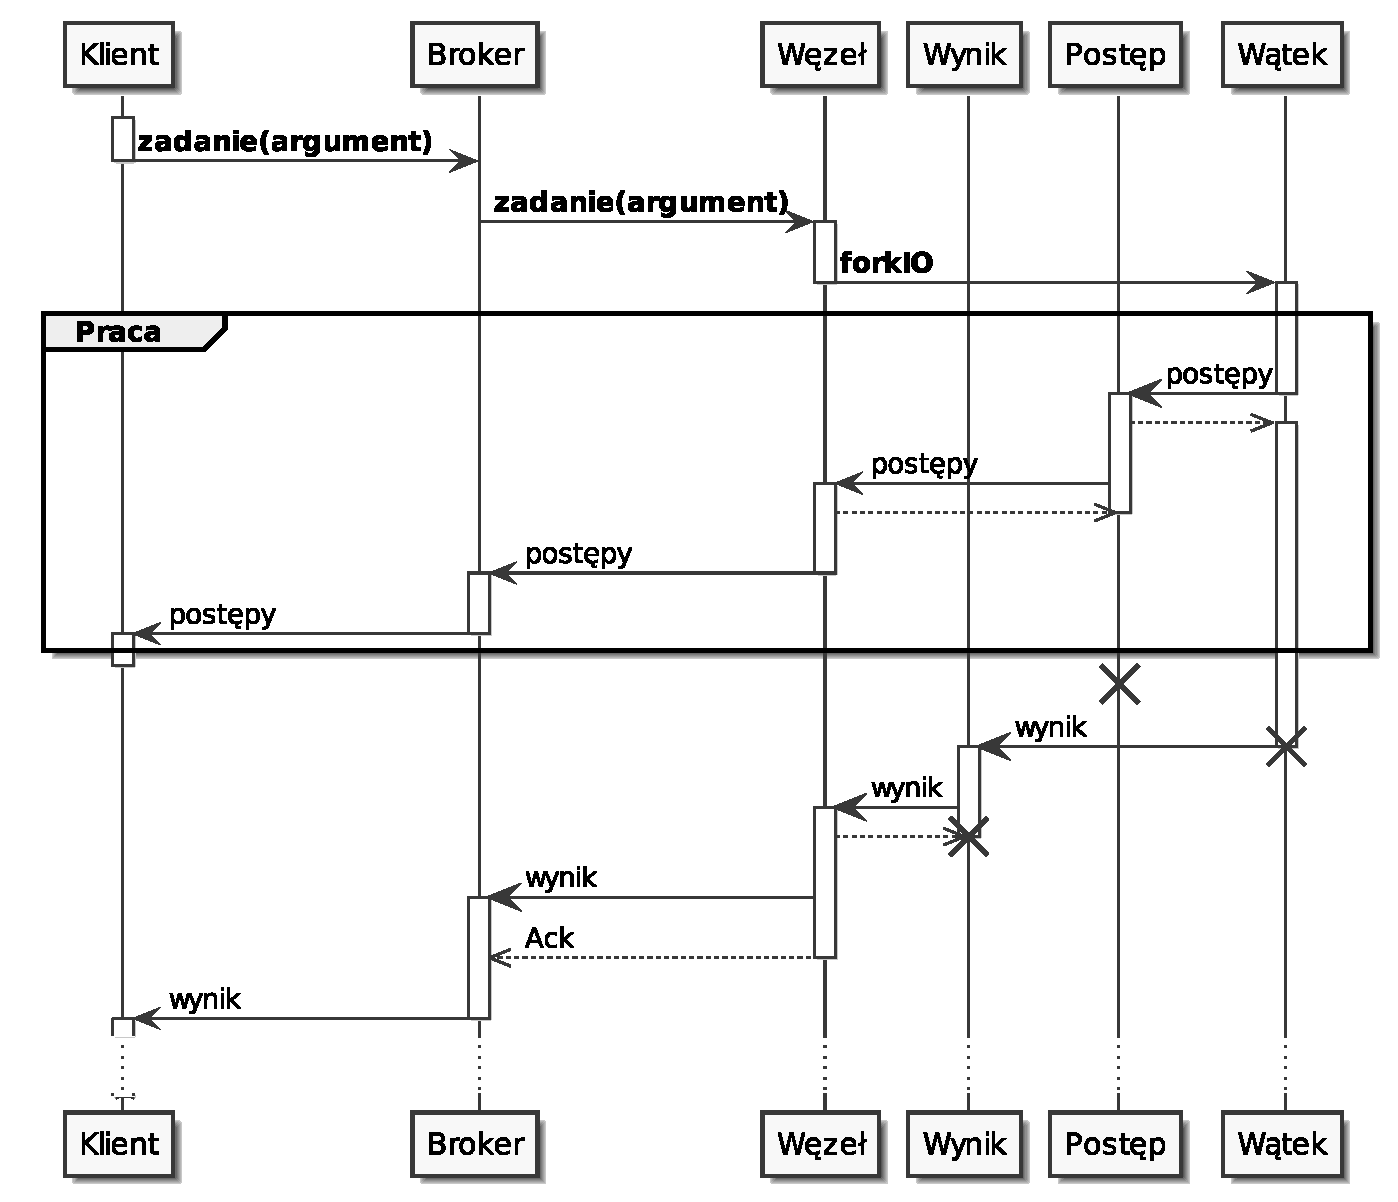
\includegraphics[width=0.8\textwidth]{sekwencja}
  \end{center}
\caption{Diagram sekwencji wykonywania zadania}
\label{fig:seq}
\end{figure}
\newpage
Kiedy postępy są zapisywane w zmiennej transakcyjnej, wykonanie wątku jest przerywane tylko na czas tego konkretnego zapisu, a przesył postępów odbywa się w innym wątku. Takie podejście minimalizuje przestoje, przy założeniu, że wysyłanie oczekujących komunikatów odbywa się szybciej niż produkcja nowych. W przeciwnym wypadku następuje blokowanie przy próbie zapisu do zmiennej, z której inny wątek nie zdążył jeszcze pobrać wartości. Obsługa przesyłania rezultatu zadania jest identyczna z obsługą postępów, co w przyszłości umożliwia zaimplementowanie zadań produkujących więcej niż jeden wynik. 

Zatwierdzenie odebrania zadania odbywa się dopiero po odesłaniu wyniku, co pozwala na wykorzystanie wbudowanego w RabbitMQ mechanizmu automatycznego ponownego kolejkowania niedokończonych zadań, na wypadek np. fizycznej awarii węzła.

\section{Przerywanie zadań}
\label{sec:przer}
Przerywanie zadań jest obsługiwane poprzez zapamiętanie identyfikatora wątku zadania w transakcyjnej mapie \cite{STMMap}, gdzie kluczami są identyfikatory aktualnie wykonywanych zadań, a wartościami identyfikatory wątku obsługującego zadanie. Komunikat przerwania zadania zawiera identyfikator zadania, które ma zostać przerwane, co umożliwia przerwanie odpowiedniego wątku. Przykładową implementację zawiera listing~\ref{lst:abort}
\begin{lstlisting}[caption=Przerywanie zadań, label=lst:abort]
type CurrentTasks = STM.Map UUID ThreadId

abortHandler :: CurrentTasks -> ReaderT (Env (Message, Envelope)) IO ()
abortHandler currentTasks = do
  Env r log (msg, env) <- ask
  deferAck r env

  let Just taskId = fromASCIIBytes $ BL.toStrict (msgBody msg)
  log $ "Got abort for task " <> toText taskId

  let strategy k = return (k, STM.Focus.Remove)
  abortCurrent <- atomically $ STM.focus strategy taskId currentTasks
  case abortCurrent of
    Just threadId -> do
        liftIO $ killThread threadId
        log "Abort received, thread killed"
    Nothing -> log "Not my task, skipping"
\end{lstlisting}
\newpage
\section{Klient}
Uruchamianie zadań jest możliwe za pomocą funkcji \lstinline{enqueueTask}, a oczekiwanie na wyniki i postępy umożliwiają odpowiednio funkcje \lstinline{onResult} oraz \lstinline{onProgress} zdefiniowane następująco:

\begin{lstlisting}[caption=Klient uruchamiający zadania]
enqueueTask :: (MonadIO m, MonadReader (Env Channel) m) 
            => T.Text -> T.Text -> BL.ByteString -> m UUID
enqueueTask qname taskName taskArgs = do
  taskId <- liftIO nextRandom
  queue newQueue { queueName = qname, queueDurable = False
                 , queueExclusive = True} $ do
    publish newMsg { msgBody = taskArgs
                    , msgID = Just $ toText taskId
                    , msgType = Just taskName
                    , msgDeliveryMode = Just Persistent }
  return taskId

onSuffix :: (MonadIO m, MonadReader (Env Channel) m) 
         => T.Text -> UUID -> (BL.ByteString -> ReaderT (Env Channel) IO ()) 
         -> m () 
onSuffix suffix taskId callback = do
  env <- ask
  queue newQueue { queueName = toText taskId <> suffix
                 , queueAutoDelete = True} $
    subscribe Ack $ do
      Env r _ (msg, envelope) <- ask
      deferAck r envelope
      liftIO $ runReaderT (callback $ msgBody msg) env
  return ()

onProgress = onSuffix ".progress"
onResult = onSuffix ".result"

\end{lstlisting}

Uruchomienie zadania polega na umieszczeniu na wybranej przez użytkownika kolejce komunikatu zlecającego zadanie, którego nasłuchują węzły. Kiedy węzeł odeśle postęp lub rezultat, możliwe jest zlecenie kolejnego zadania, w szczególności wykorzystującego rezultat poprzedniego jako swój argument. Dzięki niskopoziomowemu interfejsowi możemy wykorzystywać wiele różnych strategii serializacji i deserializacji przesyłanych danych oraz eliminować ich izomorficzne przekształcenia (niepotrzebne transformacje danych będących w odpowiednich formatach). Kosztem takiego rozwiązania jest brak bezpieczeństwa typów.

Przykład uruchamiający zadanie, wykorzystujący do serializacji bibliotekę \texttt{store} został zawarty na listingu~\ref{lst:example}
\newpage
\begin{lstlisting}[caption=Uruchamianie zadania, label=lst:example]
{-# LANGUAGE ViewPatterns #-}

deserialize :: Store a => BL.ByteString -> a
deserialize = decodeEx . BL.toStrict

serialize :: Store a => a -> BL.ByteString
serialize = BL.fromStrict . encode

printL :: (MonadIO m, Show a) => a -> m ()
printL = liftIO . print

main :: IO ()
main = logger defaultLoger $ connection "localhost" "/" "guest" "guest" $ do
  channel "task" $ do
    task1 <- enqueueTask "taskell.q1" "additionTask" 
                               $ serialize (1 :: Int, 2 :: Int)
    task1 `onProgress` \(deserialize -> p) -> printL (p :: Int)
    task1 `onResult` \r -> do
      task2 <-  enqueueTask "taskell.q1" "dummyTask" r
      task2 `onResult` \(deserialize -> p) -> printL (p :: Int)
\end{lstlisting}